\chapter{Baza podataka Firebase}

Firebase je sveobuhvatna platforma za mobilni i web razvoj koju pruža tvrtka \textit{Google}. Nudi širok raspon usluga i alata koji programerima pomažu u izradi i upravljanju aplikacijama bogatim značajkama. Firebase pruža pozadinsku infrastrukturu i usluge spremne za korištenje koje obrađuju različite aspekte razvoja aplikacija, uključujući pohranu podataka, autentifikaciju, komunikaciju u stvarnom vremenu te analitiku. Jedan segment ove platforme je \textit{Firebase Realtime Database}. To je NoSQL baza podataka koja se nalazi u oblaku. Dizajnirana je za pohranjivanje i sinkronizaciju podataka u stvarnom vremenu između klijenata i poslužitelja, što ga čini idealnim za stvaranje aplikacija u stvarnom vremenu. \cite{firebase}

U nastavku su navedene i opisane ključne mogućnosti baze podataka Firebase:
\begin{enumerate}
	\item Sinkronizacija podataka u stvarnom vremenu
	\subitem Jedna od ključnih značajki ove baze podataka jest njezina sposobnost sinkronizacije podataka u stvarnom vremenu preko povezanih klijenata. Sve promjene u bazi podataka trenutačno se prenose na sve povezane uređaje, omogućujući ažuriranje i suradnju u stvarnom vremenu.
	\item Podatkovni model NoSQL
	\subitem Ova baza podataka slijedi model NoSQL, što znači da pohranjuje podatke u strukturi nalik JSON podacima koja se sastoji od parova ključ-vrijednost. Ova fleksibilna shema omogućuje jednostavnu i dinamičnu pohranu podataka, kao i ugniježđivanje podatkovnih objekata i nizova.
	\item \textit{Offline} način rada
	\subitem Firebase pruža ugrađenu izvanmrežnu podršku, omogućujući aplikacijama da nastave funkcionirati čak i kada je uređaj izvan mreže ili ima povremenu vezu. Promjene podataka izvan mreže automatski se sinkroniziraju s poslužiteljem nakon ponovnog uspostavljanja veze.
	\item Autentifikacija
	\subitem Firebase nudi ugrađene usluge provjere autentičnosti koje osiguravaju bazu podataka omogućavaju kontrolu nad pristupom podacima. Za autentifikaciju korisnika također mogu se koristiti vanjski pružatelji usluga. Sigurnosna pravila mogu se definirati za radi detaljne kontrole pristupa i validacije. 
	\item Skalabilnost
	\subitem Ova baza podataka pruža mogućnost raspršivanja podataka na više instanci baze, što omogućava prilagodbu rastućim zahtjevima na sustav i povećanju opterećenja, zadržavajući performanse, pouzdanost i učinkovitost.
	\item Postojanost podataka
	\subitem Firebase automatski zadržava podatke na disku, osiguravajući da podaci ostanu dostupni čak i ako se aplikacija ponovno pokrene ili se uređaj isključi.
	\item Pretplata na događaje u stvarnom vremenu
	\subitem Moguće je postaviti pretplatnike na događaje promjene stanja u bazi na željenim stazama podataka. Ovo omogućuje aplikacijama da reagiraju i ažuriraju se u stvarnom vremenu kada dođe do promjene podataka. Događaji se mogu koristiti za praćenje promjena podataka.
	\item Integracija s ekosustavom Firebase
	\subitem Ova se baza podataka neprimjetno integrira s drugim uslugama u sklopu platforme, što omogućuje izradu \textit{end-to-end} aplikacija koristeći paket usluga u sklopu platforme Firebase.
\end{enumerate}

Na slici \ref{fig:firebase_integration} nalazi se pregled proizvoda koje je moguće integrirati u projekt korištenjem baze podataka Firebase.

\begin{figure}[ht]
	\centering
	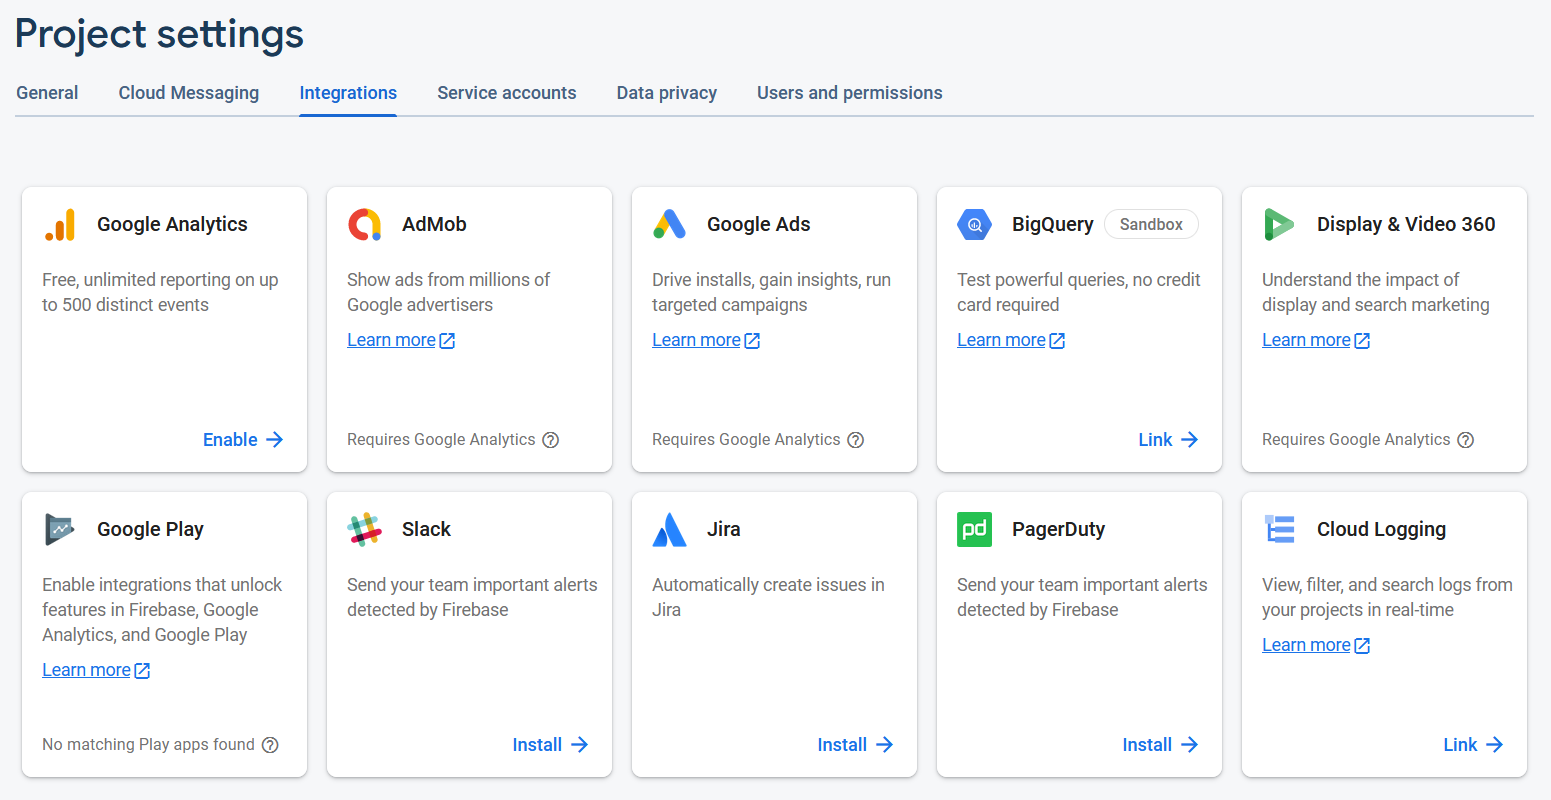
\includegraphics[scale=0.4]{imgs/firebase_integration}
	\caption{Mogućnosti integracije baze podataka Firebase s drugim proizvodima \cite{firebase}}
	\label{fig:firebase_integration}
\end{figure}

NoSQL baze podataka nisu bazirane na relacijskom modelu podataka, stoga upitni jezik SQL, koji je standardni upitni jezik za relacijske baze podataka, uglavnom nije u takvim sustavima zastupljen. NoSQL sustavi nastali su iz novih zahtjeva za većom fleksibilnošću i boljim performansama u pohrani i obradi velike količine podataka, uglavnom zbog popularnosti interneta i internetskih tehnologija te sve veće količine podataka. \cite{nosql} Koriste različite podatkovne modele za pristup i upravljanje podacima, kao što su dokumenti, grafovi, parovi ključ-vrijednost i pretraživanje. Ove vrste baza podataka posebno su optimirane za aplikacije koje zahtijevaju veliku količinu podataka, nisku latenciju i fleksibilne modele podataka. \cite{wat_zijn_nosql}

Kao što je navedeno, model Firebase baze podataka temeljen je na parovima ključ-vrijednost, gdje je jednom tekstualnom ključu pridružena jedna vrijednost bilo kojeg tipa. Takav je model podataka po strukturi sličan rječniku. Ovakve baze nemaju upitni jezik - samo omogućavaju pronalaženje, dodavanje i uklanjanje parova na osnovu ključa. Općenito, podržavaju tri operacije:
\begin{itemize}
	\item GET (ključ) - vraća vrijednost pridruženu zadanom ključu,
	\item PUT (ključ, vrijednost) - dodaje novi par ili pridružuje novu vrijednost zadanom ključu,
	\item DELETE (ključ) - uklanja par na temelju zadanog ključa.
\end{itemize}

Ključ može biti u raznim formatima, kao što je specifikacija direktorija za neku datoteku, niz znakova koji predstavlja jedinstven kod, poziv mrežnog servisa REST ili internetska stranica. Vrijednosti pridružene ključu također mogu biti raznolike, kao što su slike, zvuk, internetske stranice ili dokumenti.

Za ovakve baze podataka općenito vrijede sljedeća pravila:
\begin{itemize}
	\item svaki ključ u tablici mora biti jedinstven,
	\item nema upita na osnovu vrijednosti, samo na osnovu ključa.
\end{itemize}

Prednosti ovakvog sustava jest jednostavnost koja se očituje u performansama i skalabilnosti. Budući da se koriste jednostavne operacije, podaci se mogu modelirati tako da se maksimalno iskoristi efikasnost ovakvog sustava.

Svi podaci u bazi podataka \textit{Firebase Realtime Database} pohranjuju se kao JSON objekti, čime se stvara JSON stablo koje se nalazi u oblaku. Dodavanjem podataka u JSON stablo, podatak čvor u postojećoj JSON strukturi s pridruženim ključem. Mogu se koristiti vlastiti ključevi, primjerice jedinstveni identifikatori ili semantička imena, ili vam se mogu automatski pridružiti. Vlastiti ključevi ne smiju sadržavati specijalne znakove i moraju iznositi maksimalno 768 bajtova. Sljedeći isječak prikazuje primjer jednog ulaznog podatka u bazi Firebase. U ovom primjeru, ulazni podatak sadrži objekt \lstinline|users| koji unutar sebe ima ugniježđene objekte. Iako baza podataka koristi JSON stablo, podaci pohranjeni u bazi mogu se predstaviti kao određeni izvorni tipovi koji odgovaraju dostupnim JSON tipovima poput \textit{string}, \textit{boolean} i \textit{integer}.

\begin{lstlisting}[caption={Primjer jednog podatka u bazi Firebase}]
{
	"users": {
		"socrates": {
			"name": "Socrates",
			"contacts": { "aristotel": true },
		},
		"aristotel": { ... },
		"plato": { ... }
	}
}
\end{lstlisting}

Iako Firebase dopušta ugniježđivanje podataka do dubine od 32 razine, ugniježđivanje je preporučljivo izbjegavati. Kada se dohvaćaju podaci iz baze podataka, također se dohvaćaju sve njezini podređeni čvorovi, što znatno usporava dohvat podataka ako je velika dubina ugniježđenosti. Osim toga, pruživši nekome pristup za čitanje ili pisanje na čvoru, pružen je pristup svim podacima u tom čvoru, uključujući podčvorove. Stoga je u praksi najbolje zadržati strukturu podataka što ravnijom, odnosno odvojiti logičke cjeline u pojedine indekse. Indeksi su grupe podataka analogne tablicama u relacijskom modelu baza. U sljedećem je isječku prikazan primjer pravilnog kreiranja indeksa.  

\begin{lstlisting}[caption={Primjer kreiranja dva indeksa}]
// An index to track Ada's memberships
{
	"users": {
		"socrates": {
			"name": "Socrates",
			// Index Socrates's groups in his profile
			"groups": {
				// the value here doesn't matter, just that the key exists
				"greatphilosophers": true,
				"techpioneers": false
			}
		},
		...
	},
	"groups": {
		"greatphilosophers": {
			"name": "Great Historical Philosophers",
			"members": {
				"socrates": true,
				"aristotel": true,
				"plato": true
			}
		},
		"techpioneers": {
			"name": "Historical Tech Pioneers",
			"members": {
				"ntesla": true,
				"tedison": true,
				"agbell": true
			}
		},
	...
	}
}
\end{lstlisting}

Gore prikazanim pristupom dupliciraju se neki podaci, te pri uklanjanju jednog korisnika moraju se izmijeniti dva indeksa. Ovo je nužna redundantnost za dvosmjerne odnose. Omogućuje brzo i učinkovito dohvaćanje podataka, čak i kada se popis korisnika ili grupa povećava na milijune ili kada sigurnosna pravila baze podataka u stvarnom vremenu sprječavaju pristup nekim zapisima. 

\eject